%\doublespacing

\newcommand{\AUTHOR}{%
Xi He\\
Service Oriented Cyberinfrastruture Lab, Rochester Institute of Technology\\
~Bldg 74, Lomb Memorial Drive, Rochester, NY 14623-5608 \\
~xi.he@mail.rit.edu%
}
\newcommand{\TITLE}{A Report on Green Data Centers}

%\TABLEOFCONTENTS

\title{\TITLE}
\author{\AUTHOR}

\maketitle

\begin{abstract}
This report is targeted on presenting the state of art research progress of making data centers green. A brief introduction of data centers is first presented, and then metrics for measuring the energy efficiency of data centers are thoroughly examined. The primary focus of this report aims to review and categorize the recent research progress in Green Computing, specially on reducing the energy cost in data centers. This report also describes a few related project and implementation.

\end{abstract}

%%%%%%%%%%%%%%%%%%%%%%%%%%%%%%%%%%%%%%%%%%%%%%%%%%%%%%%%%%%%%%%%%%%%%%
\section{Introduction}
%%%%%%%%%%%%%%%%%%%%%%%%%%%%%%%%%%%%%%%%%%%%%%%%%%%%%%%%%%%%%%%%%%%%%%
A data center, also called a server farm, is a facility housing computer systems and associated components, such as telecommunication and storage systems. A typical data center is composed of 
\begin{itemize}
\item IT equipment, including servers, storage devices and network devices.
\item Heating, ventilating and air conditioning system (HVAC).
\item Backup power, including uninterruptible power supplies (UPS) and diesel generators.
\item Fire protection system.
\item Physical security system.
\end{itemize}

Back to the early ages of the computing industry, the computer systems were too complex to operate and maintain, and required a special environment in which to operate. Those huge computer rooms at that time are the prototypes of modern data centers. During the boom of microcomputer industry, computers started to be deployed everywhere with little care about the operating requirements. However, as information technology operations started to grow in complexity, especially with the emerge of client-server computing, browse-sever computing and dot-com bubble, large data centers are built to provide businesses with a range of solutions for system deployment and operation.

However, with the emergence of cloud computing and high performance data centers, large energy consumption in data centers has become a challenging problem. According to U.S. Environmental Protection Agency (EPA), 61 billion kilowatt-hours of power was consumed in data center in 2006, 
that is 1.5 percent of all US electricity consumption costing around \$4.5 billion. In fact, the energy consumption in data 
centers doubled between 2000 and 2006 and EPA estimates that the energy usage will double again by 2011\cite{report/epa}. 

Figure \ref {F:trend} compares the purchasing dollars spent on new servers with power and cooling costs since 1996 and projects those number until 2010. The data illustrates that for \$1 of new 
server spend in 2005, \$0.48 was spent on power and cooling. This is a sharp 
increase from 2000, when the ratio was \$1:\$0.21. In 2010, it is projected that this ratio 
will rise to \$1:\$0.71. 

 \FIGURE{!h}
  {images/idc}
  {1.08}
  {Data Center Power \& Cooling Trend \cite{scaramella-worldwide} }
  {F:trend}

This paper sums up a a variety of industrial and academic effort of making green data centers that use computing resource in an efficient way and have little hazardous impact on the environment.
%%%%%%%%%%%%%%%%%%%%%%%%%%%%%%%%%%%%%%%%%%%%%%%%%%%%%%%%%%%%%%%%%%%%%%
\section{Data Center Basics}
%%%%%%%%%%%%%%%%%%%%%%%%%%%%%%%%%%%%%%%%%%%%%%%%%%%%%%%%%%%%%%%%%%%%%%
Data centers are the very complex system that house thousands of IT equipment and keep them continually running while consuming tremendous electrical power. A large portion of electrical consumption is used to power on the IT equipment. The cooling system consumes another increasing portion of electrical consumption to keep IT equipment in a  appropriate temperature and humidity, and remove the heat produced by IT equipment. Here we divide data center system into three parts: power subsystem, heat removal subsystem and computer room subsystem, and illustrate each part in detail.

\subsection{Power Subsystem}
\begin{figure*}[ht!]
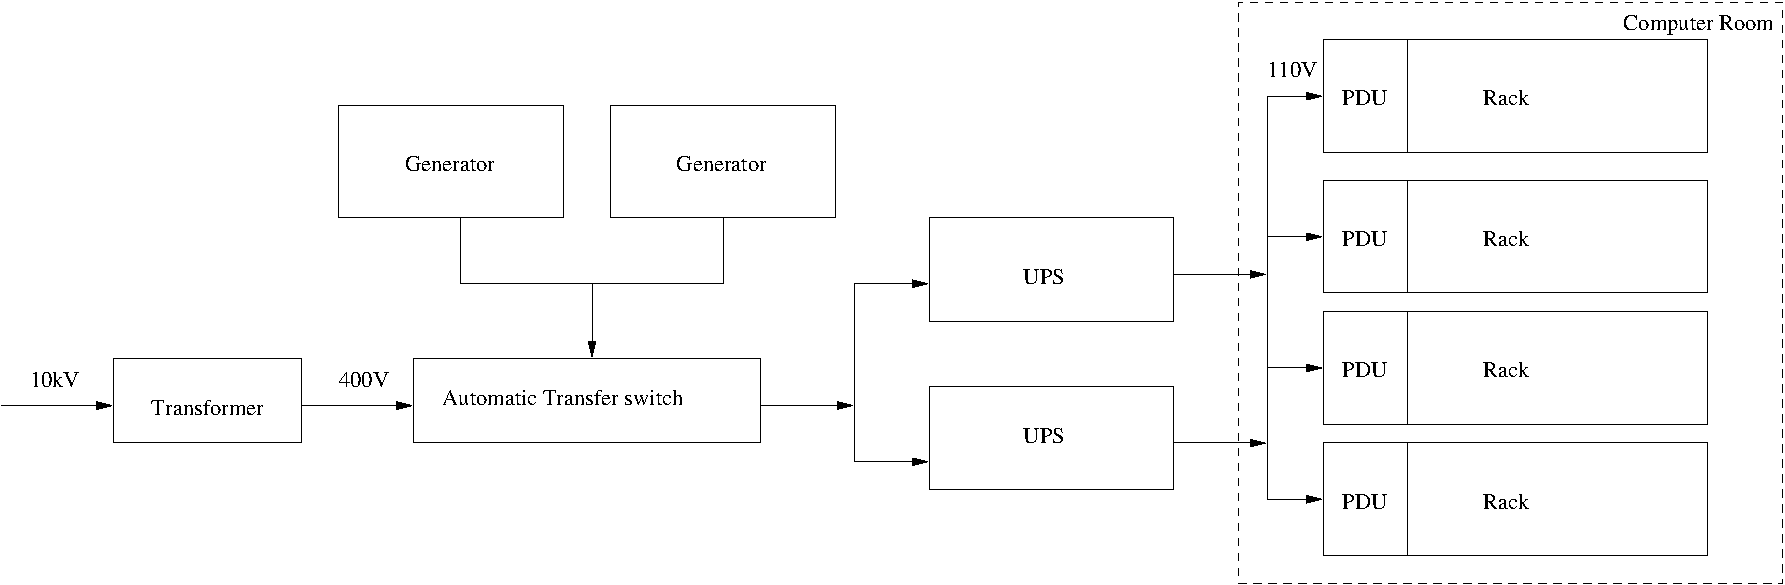
\includegraphics [totalheight=0.24\textheight]{images/power}
\caption {A typical power subsystem}
\label {F:power}
\end{figure*}

Figure \ref{F:power} shows a typical power system. Power (10--20kV) enters the building from the utility's substation. After passing the {\em transformer} which turns the voltage from 10-20kV to 400-600kV, the power is distributed to {\em UPS} (Uninterruptible power supply) by {\em automatic transfer switch}. A set of diesel generators act as a second power feed when utility power fails. The {\em UPS} output is then routed to {\em PDUs} (Power Distribution Units) that sit in data center room.  The {\em PDUs} take a higher voltage feed (200-480kV) and break it up into the many 110V circuits that feed the actual server.

\subsection{Heat Removal Subsystem} 
Almost all of the power dissipated in a data center is converted to heat, which must be evacuated from the facility. As shown in Figure \ref{F:cooling}, {\em CRACs} transfer the heat from servers' hot exhaust to a chilled water loop. The water heated by {\em CRACs} is then pumped into a {\em Chiller} where heat is exchanged between the inner water loop and a second loop connected to a cooling tower, where heat is released to the outside atmosphere. The cooled water from the cooling tower is routed back to {\em CRACs}.

\begin{figure*}[ht!]
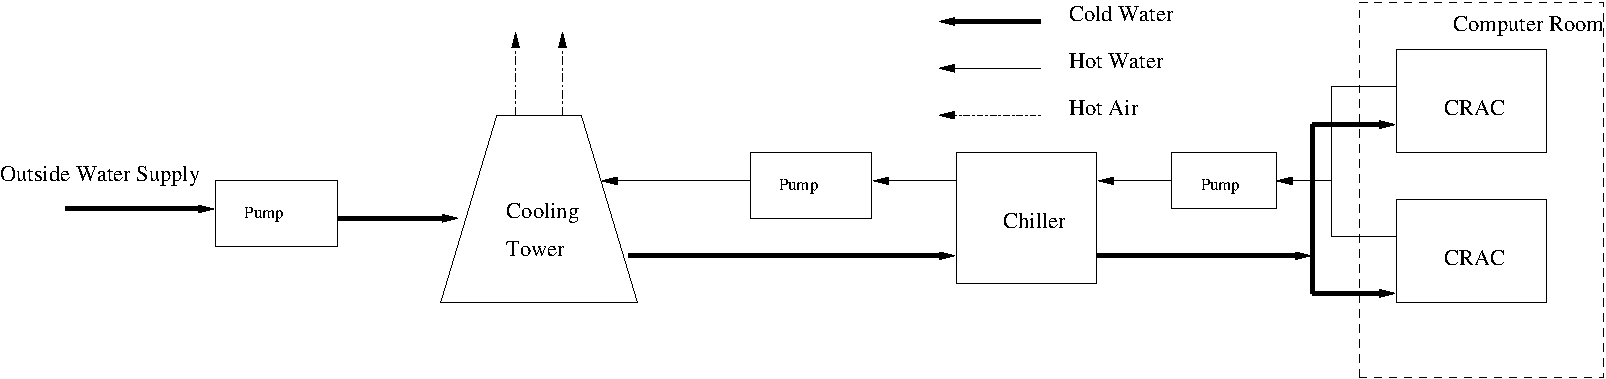
\includegraphics [totalheight=0.18\textheight]{images/cooling}
\caption {A typical heat removal subsystem}
\label {F:cooling}
\end{figure*}

\subsection{Computer Room Subsystem} 
\FIGURE{htb}
 {images/datacenter3}
 {1}
 {The typical architecture of data centers}
 {F:f1}

Figure \ref{F:f1} shows how a data center is organized.  The racks are laid out in rows on a raised floor over a shared plenum, and arranged back-to-back so that cool aisles and hot aisles are formed to minimize air mixing and increase cooling efficiency. Computer room air conditioning(CRAC) units along the walls take in the re-circulated exhaust hot air, cool the air over a refrigerated or chilled 
water cooling coil to approximately 10-17$^\circ$ and direct the cooled air into the shared plenum. 
%%%%%%%%%%%%%%%%%%%%%%%%%%%%%%%%%%%%%%%%%%%%%%%%%%%%%%%%%%%%%%%%%%%%%%
\section{Metrics}
%%%%%%%%%%%%%%%%%%%%%%%%%%%%%%%%%%%%%%%%%%%%%%%%%%%%%%%%%%%%%%%%%%%%%%

%---------------------------------------------------------------------
\subsection{DCiE~\&~PUE}
%---------------------------------------------------------------------


In 2007, The Green Grid\cite{thegreengrid} proposed two data center efficiency metrics: DCiE (Data Center Infrastructure Efficiency) and its reciprocal, PUE (Power Usage Effectiveness)\cite{report/greengridreport3}. 

\begin{equation}
\mathrm {DCiE} =  \frac { \textrm {IT Equipment Power} }  {\textrm {Total Facility Power} }
\end{equation}

\begin{equation}
\mathrm {PUE} = \frac {1} {\textrm {DCiE}} =\frac {\textrm {Total Facility Power}} { \textrm {IT Equipment Power} }
\end{equation}

%A phased approach will be adopted as The Green Grid\cite{thegreengrid} provides increasingly detailed information with respect  to quanti�cation of the DCiE.  Table \ref {T:dcie}  provides a graphical representation of the approach (PDU=Power Distribution Unit, UPS=Uninterruptible Power Supply, HVAC=High Voltage Alternating Current. )

%\begin{table*}[ht]
%\caption{A phase approach for DCiE measurement }
%\begin{center}
%\begin{tabular}{|c|c|c|c|}
%\hline
%& Level 1  & Level 2   & Level 3   \\
%\hline 
%  IT equipment power     &  UPS   &PDU   & server, rack, router   \\
% 
%\hline 
%Total   facility power & Data Center    input power & Data Center   input power   & Data Center input power \\
%& input power & less shared HVAC & Less shared HVAC \\
%& & & plus building light, security\\
%\hline 
%interval & \~{} 1 week  &   \~{}  1 day& \~{} 1 minute  
%\\
%\hline

%\end{tabular}
%\end{center}
%\label{T:dcie}
%\end{table*}%

\begin{itemize}

\item {\em IT Equipment Power:} This includes the load associated with all of the IT equipment, 
i.e. compute, storage and network equipment,  along with supplemental equipment i.e. 
KVM switches, monitors, and workstations/laptops used to monitor or otherwise control the data center. 

\item  {\em Total Facility Power:} 
This includes all IT Equipment power as described above plus everything that supports the IT 
equipment load such as: 

\begin{itemize}

\item  Power delivery components i.e. UPS, switch gear, generators, PDUs, 
batteries and distribution losses external to the IT equipment 

\item  Cooling system components i.e. chillers, computer room air conditioning  
(CRAC) units, direct expansion air handler (DX) units, pumps, and cooling towers 

\item  Other miscellaneous component loads such as datacenter lighting 

\end{itemize}

\end{itemize}

Both PUE and DCiE provide a scale for measuring a data center's operational efficiency. Take PUE for example, a PUE of 2.0 
indicates that for every watt of IT power, an additional watt is consumed to cool and distribute power to the IT equipment. The PUE of a typical enterprise data center is around between 1 to 3. Some preliminary work indicates that many datacenters may 
have a PUE of 3.0 or greater, but with proper design a PUE value of 1.6 should be achievable. This theory 
is supported by measurements completed by Lawrence Berkley National Labs\cite{greenberg2006best} which shows that the 22 
datacenters measured had PUE values in the 1.3 to 3.0 range. Other research indicates that PUE values of 
2.0 are achievable with proper design\cite{report/upssilicon}. However, there is currently no comprehensive industry data set that 
shows accurate PUE statistics for datacenters. 


 Figure \ref{F:pue} shows examples of PUE curves for various hypothetical data centers, wherein $m_{PUE}$ is the linear slope of proportional scalability for a given statistical mean PUE value. 

 \FIGURE{!h}
  {images/pue.pdf}
  {1.0}
  {PUE scalability}
  {F:pue}


%---------------------------------------------------------------------
\subsection{DCeP}
%---------------------------------------------------------------------


DCP (Data Center Productivity)\cite{report/greengridreport6} is a class of metrics that quantify the useful work that a data center produces in relation to the resource it consumes. DCeP (Data Center Energy Productivity)\cite{report/greengridreport6} is a member of the DCP metrics family.  It accounts for the energy productivity of a data center to produce the useful work.

\begin{equation}
DCeP = \frac {\textrm{Useful Work}}
{\textrm{Total Energy Consumed To Produce That Work }}
\end{equation}

Useful work may be defined as follows:

\begin{equation}
\textrm{Useful Work} = \sum^{M}_{i=1}Vi*U_i(t,T)*T_i
\end{equation}

Where $M$ is the number of tasks initiated during the assessment window, and 
$V_i$ is a normalization factor that allows the tasks to be summed numerically. $T_i = 1$ if task i completes during the assessment window, and 
 $T_i= 0$ otherwise. $U_i(t,T)$ is a time-based utility function for each task, where the parameter $t$ is elapsed time from initiation to completion of the task, and $T$ is the absolute time of completion of the task.
 
 The equation is complex and difficult to measure, and some terms require user interpretation. A simplification may be made to transactional or throughput-based workloads:
 
\begin{equation}
\textrm{Useful Work} =\textrm{The Number of Transactions}
\end{equation}
 
For example, if a data center conducts a 375,000 request/response transactions in the 30-minute assessment window, and the total energy consumption in this period is  0.474 kWh, then the normalized tasks per kWh is 505,663. 

The DCeP is a more sophisticated metrics for people to quantify data ceters' efficiency and it is impractical for many data centers to measure DCeP. In fact the DCeP itself is still under development. As an alternate way to quantify data centers' efficiency, the {\em Green Grid} proposes a set of {\em productivity proxy} that can indicate how many work is being done without directly measuring work. For example, the proxy {\em Bits per Kilowatt-hour} sum all the outbound bitstreams from data center, and divide by energy by data centers. 
  
%%---------------------------------------------------------------------
%\subsection{Proxy for DCeP}  
%%---------------------------------------------------------------------
% 
%Proxies indicate how much work is being done without measuring work directly. They are often used where complex measures would be impractical.
% 

%%---------------------------------------------------------------------
%\subsubsection{Useful Work Self-Assessment and Reporting}  
%%---------------------------------------------------------------------
% \begin{equation}
% Proxy_{DCeP}=\frac {\sum_{i=1}^{n} N_i \times W_i }{E_{DC}}
% \end{equation}

%where: \\
% $n $ is the number of instrumented applications running during the assessment window. \\
%$ N_i $ is a normalization factor for each software application. \\
% $W_i$ is the number of units of useful work reported by a particular instrumented application. \\
% $E_{DC}$ is the total energy consumed by the data center during the assessment window. \\

%
%%---------------------------------------------------------------------
%  \subsubsection{DCeP subset by productivity link}
%%---------------------------------------------------------------------

%
%  \begin{equation}
%  Proxy_{Prod~Link}=\frac{ (\frac{N_{DC}}{N_{subset}}) \times {\sum_{i=1}^n W_i} }{E_{DC}}
%  \end{equation}

%  where: \\
% $N_{DC}$ is the total number of servers in the data center. \\
% $N_{subset}$ is the number of servers in the subset. \\
% $n$ is the number of instrumented applications running during the assessment window. \\
% $W_i$  is the number of units of useful work reported by an instrumented application. \\
% $E_DC$ is the total energy consumed by the data center during the assessment window.\\
% 
% 
% 
%%---------------------------------------------------------------------
% \subsubsection{DCeP subset by sample workload}
%%---------------------------------------------------------------------

%

%  \begin{equation}
%  Proxy_{DCePsubset}=\frac{ (\frac{N_{DC}}{N_{subset}}) \times {W_{subset}} }{E_{DC}}
%  \end{equation}

%  where: \\
% $N_{DC}$ is the total number of servers in the data center. \\
% $N_{subset}$ is the number of servers in the subset. \\
% $W_{subset}$  is the number of units of useful work reported by an instrumented application. \\
% $E_DC$ is the total energy consumed by the data center during the assessment window.\\
% 
% 

%%---------------------------------------------------------------------
%\subsubsection{Bits for Kilowatt-Hour}
%%---------------------------------------------------------------------

%
% \begin{equation}
% Proxy_{bkwh}=\frac {\sum_{i=1}^k b_i} {E_{DC}}
% \end{equation}

% where:  
% $k$ is the total number of outbound routers. \\
% $b_i$ is the total number of bits coming out of the ith router during the assessment window. \\
% $E_{DC}$ is the total energy consumed by the data center during the assessment window. \\
% 
%How to measure variables in the numerator: 
% $b_i$ is summed from traf� c statistics at all routers providing outbound traf� c from the data centers 
%during the assessment window.\\

%%---------------------------------------------------------------------
%\subsubsection{Weighted CPU Utilization SPECint\_rate}  
%%---------------------------------------------------------------------
%%---------------------------------------------------------------------
%\subsubsection{Weighted CPU Utilization SPECpower}  
%%---------------------------------------------------------------------
%%---------------------------------------------------------------------
%\subsubsection{Compute Units Per Second}  
%%---------------------------------------------------------------------
%%---------------------------------------------------------------------
%\subsubsection{Operating System Workload Efficiency}  
%%---------------------------------------------------------------------

%%%%%%%%%%%%%%%%%%%%%%%%%%%%%%%%%%%%%%%%%%%%%%%%%%%%%%%%%%%%%%%%%%%%%%
\section{IT Equipment Side}
%%%%%%%%%%%%%%%%%%%%%%%%%%%%%%%%%%%%%%%%%%%%%%%%%%%%%%%%%%%%%%%%%%%%%%

The effort of saving energy on IT equipment side aims to reduce the energy consumed by servers, storage devices and network devices. Obviously, energy savings are significant if unused IT equipments can be shut down. But this approach works only when future task arrival distribution can be predicted based on past events and the deadline for task completion is flexible, such as for the data centers housing interactive cluster-based commercial servers.  For scientific computing, more suitable approaches are needed.

\subsection{Low-power Computing}
The low-power approach has been successfully adopted in the systems that run on limited power supplies such as PDAs and laptops. Yet this approach is also  applied to high performance computing in an effort to reduce the tremendous energy consumption, including the powering and cooling cost. For example, the Japanese Earth Simulator, ranked as the top supercomputer on the TOP500 list from 2002 to 2004, consumed 12 MW of power, resulting in US\$10 million per year just for powering and cooling.  As the first supercomputing built with energy efficiency as its guiding principle, Green Destiny(http://sss.cs.vt.edu) used the nontraditional and low power processors to achieve lower power consumption and thus low temperature which means increased reliability and no cooling energy cost. However, low power processors sacrificed too much performance, and to scale up the performance, a larger number of processors are needed. For instance, IBM's Blue Gene/L uses more than 100,000 processors. 

\subsection{Power-aware Computing}

Most of the power consumption in processors is proportional to $V^2f$, where $V$ is the voltage on processors and $f$ is the processors' frequency. Since energy is defined as power multiplied by time, the energy consumed in processors is proportional to $V^2$, which means we can reduce energy consumption by lowering the voltage. On the other hand, in order for the processors to work safely, the voltage can not be decreased without a corresponding decrease of the frequency. And the frequency is inversely proportional to execution time and thus reducing the voltage results in performance loss. As a result, there is an important research issue concerning how to balance the tradeoff between energy consumption and performance penalty. 

Focusing on parallel programs, many researchers leverage dynamic voltage and frequency scaling (DVFS) technology and scale down the processors' supply voltage and frequency at appropriate times so that the energy can be conserved with little performance penalty. In \cite{chen2005reducing,kimura2006emprical}, the researchers aim to identify compute nodes and execution phases that are not on the critical execution path and then scale them down while still meeting the time constraint. As shown in Figure \ref{F:dvfs1}, a parallel program is modeled as a DAG (directed acyclic graph) with six task nodes: A, B, C, D, E, F. Task A, B, C, D is on the critical execution path, and there is no room for them to change the frequency, otherwise the total execute time would increase. For Task-C, it finishes earlier than Task-B, but the system still has to wait until Task-B finishes and then starts to execute Task-E. So there is some slack time for Task-C and energy conservation can be achieved by lowering the frequency of processor running Task-C.  Figure \ref{F:dvfs3} shows the optimized program execution scheme.  

\begin{figure*}[htb]
    \centerline{
    \subfigure[Initial program execution scheme]{\label{F:dvfs1}{\resizebox{0.5\linewidth}{!}{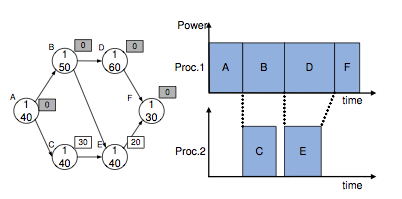
\includegraphics{images/dvfs1}}}}
    %\subfigure[b]{\label{F:dvfs2}{\resizebox{0.3\linewidth}{!}{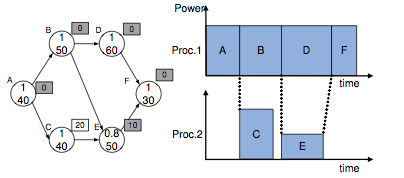
\includegraphics{images/dvfs2}}}}
    \subfigure[Optimized program execution scheme]{\label{F:dvfs3}{\resizebox{0.5\linewidth}{!}{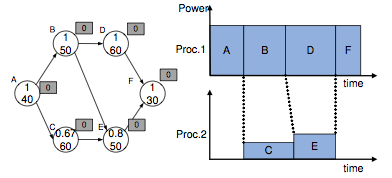
\includegraphics{images/dvfs3}}}}
    }
\caption {A DAG representing a sample parallel program and its power profile. The two numbers inside each node, from top to bottom, represent normalized frequency and the task's execution time. The box on the node indicates the slack time. \cite{kimura2006emprical}}
\label {F:dvfs}
\end{figure*}

However, the above approach requires significant effort with respect to performance profiling and program analysis and is often application-dependent; The second one leverages the identification of execution phases in an application and then schedules appropriate voltage and frequency for each phase\cite{freeh2005using,kimura2008runtime}. The third approach is similar to the second one, but the DVFS control is implemented as autonomic, performance-directed, runtime controller independent of the applications running\cite{hsu2005power,ge2007cpu}. In \cite{kim2007power,DBLP:conf/sc/GeFC05}, the researchers present their DVFS based scheduling framework.

\subsection{Server Consolidation}
Server virtualization \cite{DBLP:conf/sosp/BarhamDFHHHN03} is another way to address the large power consumption problem. Most servers and desktops today are in use only 5-15\% of the time they are powered on, yet most x86 hardware consumes 60-90\% of the normal workload power even when idle. With virtualization technique, all the VMs share the same physical resources and the utilization of the physical server can reach up to 80\% with ignorable overhead. Thus, although using virtualization results typically in a performance loss using the available hardware more efficiently provides great contribution in regards to the utilization. The work \cite{von2009power} schedules the Virtual Machines on DVFS-enabled clusters and achieves significant power consumption reduction with little performance penalty.  

%%%%%%%%%%%%%%%%%%%%%%%%%%%%%%%%%%%%%%%%%%%%%%%%%%%%%%%%%%%%%%%%%%%%%%
\section{Cooling System}
%%%%%%%%%%%%%%%%%%%%%%%%%%%%%%%%%%%%%%%%%%%%%%%%%%%%%%%%%%%%%%%%%%%%%%

Researchers usually approach the thermal management problem in two different ways. One is from the infrastructure design and planning perspective. In \cite{huang2004compact}, CFD modeling and increased deployment of temperature sensors are involved in the phase of data center design and analysis. The work in \cite{sullivan2000alternating} evaluates layout of the computing equipment in the data center to minimize air flow inefficiencies. 


The second approach is targeted on improving the cooling power efficiency by temperature-aware workload placement. Current techniques control the computer room air conditioning units (CRACs) based on the return air temperature --typically set near $20\circ C$. Blowers within the CRACs are normally operated at maximum �ow rate throughout the operation of the data center unless they are equipped with nonstandard variable frequency drives. At this setting the blowers typically provide signi�cantly more air�ow than is required by the equipment racks to prevent recirculation and the subsequent formation of 
hot spots. This strategy tends to be overly conservative and inef�cient. The experiment conducted by Timothy D. Boucher et. al.  using these CRAC setting shows that nearly 0.7W is consumed by the environmental control system for 1W of heat dissipated by the IT equipment. The study\cite{boucher2006viability} examines several opportunities for improving thermal management and energy performance of data center with automatic control. The experimental result shows that it is possible to improve the energy performance of a data center by up to 70\% while maintaining proper thermal management conditions.  In the work from HP Lab\cite{DBLP:conf/usenix/MooreCRS05}, the researchers describe the potential of temperature-aware workload plancement. As Figure \ref{F:potential} indicates, the benefits of temperature-aware workload placement are limited at the two end points -- a data center at ``0\%'' utilization or at ``100\%'' does not offer much scope for workload placement to reduce cooling costs. The benefits exist at intermediate utilization levels when we can choose how we place workload.

 \FIGURE{!h}
  {images/potential}
  {1.0}
  {Potential of Temperature-aware Workload Placement}
  {F:potential}
  
The cooling system in data centers extracts the heat produced by servers and maintains server's inlet air temperature below the redline temperature. Typically the efficiency of the cooling system depends on external environmental control which is affected  by irregular air flows and nonuniform workload. Therefore, more efficient cooling system can be achieved by appropriate workload placement. In \cite{DBLP:journals/internet/SharmaBPFC05}, based on the simulation result that there exists temperature imbalance for a row of racks, the researchers proposes to schedule the workload according to the extract temperature of the racks in a row. In \cite{DBLP:conf/cluster/TangGV07, DBLP:conf/usenix/MooreCRS05}, the researchers study the recirculation problem in data centers and propose a task scheduling algorithm to minimize heat recirculation, thus leading to minimal cooling energy cost. The shortcoming of these two approaches is that instead of compute nodes, they study compute racks which contain a certain number of compute nodes with different temperature. As a result, these solutions are less accurate than others. The more elaborate thermal aware tasks are with computational fluid dynamic (CFD) models \cite{DBLP:journals/tc/ChoiKSSWL08}. However, some research declares that CFD based model is too complex and is not suitable for online scheduling.  HP lab presents a neural network based thermal predictive model\cite{moore2006wao}. Unfortunately, no detailed information is exposed to academic community due to industry restriction. Also the thermal aware task scheduling proposed in this paper is time-consuming and impractical.    




%%%%%%%%%%%%%%%%%%%%%%%%%%%%%%%%%%%%%%%%%%%%%%%%%%%%%%%%%%%%%%%%%%%%%%
\section{Development and Implementation}
%%%%%%%%%%%%%%%%%%%%%%%%%%%%%%%%%%%%%%%%%%%%%%%%%%%%%%%%%%%%%%%%%%%%%%
\subsection{Data Center Observatory}
The Data Center Observatory (DCO)\cite{www/DCO} can provide invaluable real data to system researchers seeking to understand the sources of operational costs and a real environment to evaluate novel solutions. The DCO has been designed with detailed monitoring instrumentation at every level, on power/cooling, on the software systems and on human administration time so that it can provide users a live environment to analyze resource costs and test reasonably mature new technology and measure how well they work.

Figure \ref{F:dco} shows the DCO architecture.
 
\FIGURE{!h}
       {images/dco.pdf}
       {1.0}
       {DCO architecture}
       {F:dco}
 
\subsection{Mercury}
Mercury \cite{www/mercy} is a software suite targeted on solving the thermal problems in data centers by means of accurately emulating temperatures based on simple layout, hardware, and component utilization data. 
The main components of Mercury are:

\begin{itemize}

\item {\em Solver:} The solver is the part of the suite that actually computes temperatures using finite-element analysis. It receives component utilization data from a trace file or from monitoring daemons. 

\item {\em Monitoring daemon:} The monitor daemon, called monitord, periodically samples the utilization of the components of the machine on which it is running and reports that information to the solver. The components considered are the CPU(s), disk(s), and network interface(s) and their utilization information is computed from /proc. 

\item {\em Sensor library:} Applications and system software can use Mercury through a simple runtime library API that comprises three calls: opensensor(), readsensor(), and closesensor(). 

\item {\em Thermal emergency tool:} To simulate temperature emergencies and other environmental changes, Mercury creates a tool called fiddle. Fiddle can force the solver to change any constant or temperature on-line. 

\end{itemize}

Figure \ref {F:mercury} shows the Mercury architecture.

 
\FIGURE{!h}
  {images/mercury.pdf}
  {1.0}
  {Mercury architecture}
  {F:mercury}
 
\subsection{C-Oracle}
C-Oracle \cite{DBLP:conf/hpca/RamosB08} is a software infrastructure that allows the thermal management policy of an Internet service to predict the implications of different potential reactions to a thermal emergency.

Figure \ref {F:c-oracle} shows the Mercury architecture.

 
\FIGURE{!h}
  {images/c-oracle.pdf}
  {1.0}
  {C-Oracle architecture (TM= Thermal Management)}
  {F:c-oracle} 
\subsection{ThermoStat}
ThermoStat \cite{DBLP:journals/tc/ChoiKSSWL08, www/thermostat} is a detailed 3-dimensional Computational Fluid Dynamics tool for thermal modelling of rack-mounted server systems. The ThermoStat is based on CFD (Computational Fluid Dynamics) tools. Most academic institutions have licenses for popularly used CFD software such as FLUENT, FLOTHERM \cite{flotherm}, Phoenics etc.   Currently ThermoState is built on Phoenics (which is one of various CFD tools). ThermoStat provides useful tools for modeling and analyzing thermal behavior of rack-mounted servers and individual server.

\subsection{HP Work}
HP Lab has done impressive work on green data centers

\begin{itemize}

\item  {\em Thermal Logic}
Thermal Logic \cite{report/thermal-logic}, a portfolio of tools, can give HP BladeSystem users  more precise control over power and cooling. Thermal Logic is a set of energy measurement and management technologies HP has built into its products, and includes several new wrinkles for data center managers:

\begin{itemize}

\item HP Dynamic Power Capping, which allows companies to control the amount of power used by each server, which can reduce costly over-provisioning of power. 

\item A new cooling architecture, HP Parallel Redundant Scalable Enterprise Cooling (PARSEC), which divides each BladeSystem enclosure into multiple zones with dedicated fans, allowing users to make better use of variable fan speeds. This allows custom configurations for servers and storage, rather than adapting all fans to one high-powered blade.

\item HP Active Cool fans, which feature a new design based on aircraft technology that the company says can cool 16 blades using just 100 watts of power. 
\end{itemize}

\item {\em HP Dynamic Smart Cooling:}
HP  Dynamic Smart Cooling \cite{hp-dmc} combines sensors with control nodes that monitor temperatures in parts of the data center. These nodes control the computer room air conditioners for better control of the whole IT environment, so you do not have to cool a whole room for a few racks in one area. For example, using HP's Dynamic Smart Cooling, HP Labs reduced the power to cool a data center by anywhere from 30 to 60 percent, depending on facility infrastructure.

\item {\em CFD based simulation for thermal-awared data center management:}
HP follow Chandrakant D. Patel  leads a group of thermal-awared data center management with CFD models. 
A set of reports are released \cite{journals/dpd/BeitelmalP07, DBLP:journals/internet/SharmaBPFC05}. 
Their work can be used for designing data centers.
It is declared that CFD model is not suitable for online scheduling due to its complexity.

\end{itemize}

%%%%%%%%%%%%%%%%%%%%%%%%%%%%%%%%%%%%%%%%%%%%%%%%%%%%%%%%%%%%%%%%%%%%%%
%\section{Conclusion}
%%%%%%%%%%%%%%%%%%%%%%%%%%%%%%%%%%%%%%%%%%%%%%%%%%%%%%%%%%%%%%%%%%%%%%

%Put your conclusions in this section